% PART 3 (SECTION 8.3)
\part{Section 8.3}
%%%%%%%%%%%%%%%%%%%%%%%%%%%%%%%%%%%%%%%
\begin{transitionframe}
    \begin{center}
    { 
        \Huge \textcolor{white}{\textbf{Area and Perimeter}}
        \\[-1em]
        \noindent\textcolor{white}{\rule{12cm}{0.4pt}}
        
        %\large \textcolor{white}{Section 8.3}
    }
    \end{center}
\end{transitionframe}
%%%%%%%%%%%%%%%%%%%%%%%%%%%%%%%%%%%%%%%
%        SLIDE 
%%%%%%%%%%%%%%%%%%%%%%%%%%%%%%%%%%%%%%%
\begin{frame}{Outline}
            \tableofcontents[part=3]
\end{frame}
%%%%%%%%%%%%%%%%%%%%%%%%%%%%%%%%%%%%%%%
%        SLIDE 
%%%%%%%%%%%%%%%%%%%%%%%%%%%%%%%%%%%%%%%
\section{Perimeter}
\begin{frame}[t]{Perimeter}
    \begin{columns}
    %
    \column{0.45\textwidth}
    %
    \begin{block}{Definition}
        Perimeter, denoted $P$, is the distance around the outside of a shape.
    \end{block}
    %
    \begin{itemize}
        \item In other words, the sum of lengths of the sides of a shape.
        \item The unit of the perimeter is the same as the unit of the length such as inches (in), feet (ft), meter (m), millimeter (mm), centimeter (cm) and so forth.
    \end{itemize}
    %
    \column{0.45\textwidth}
    \textbf{Example:}
    \begin{figure}[H]
        \centering
        

\tikzset{every picture/.style={line width=0.75pt}} %set default line width to 0.75pt        

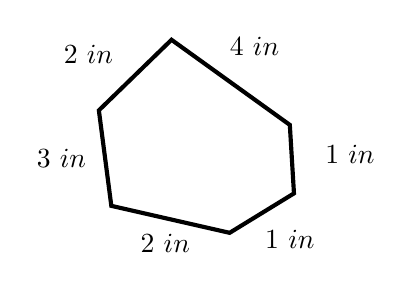
\begin{tikzpicture}[x=0.75pt,y=0.75pt,yscale=-1,xscale=1]
%uncomment if require: \path (0,167); %set diagram left start at 0, and has height of 167

%Shape: Polygon [id:ds1989494780526837] 
\draw  [line width=1.5]  (299,40) -- (356,81) -- (358,114) -- (327,133) -- (270,120) -- (264,74) -- cycle ;

% Text Node
\draw (259,47) node   {$2\ in$};
% Text Node
\draw (296,138) node   {$2\ in$};
% Text Node
\draw (246,97) node   {$3\ in$};
% Text Node
\draw (339,43) node   {$4\ in$};
% Text Node
\draw (385,95) node   {$1\ in$};
% Text Node
\draw (356,136) node   {$1\ in$};


\end{tikzpicture}
        \label{fig:perimeter}
    \end{figure}
    %
    \[
        P = 1+1+2+2+3+4 = 13\ \mathrm{in}
    \]
    \end{columns}
\end{frame}
%%%%%%%%%%%%%%%%%%%%%%%%%%%%%%%%%%%%%%%
%        SLIDE 
%%%%%%%%%%%%%%%%%%%%%%%%%%%%%%%%%%%%%%%
\begin{frame}[t]{Example (Find the perimeter)}
    \begin{example}
        Find the perimeter of the following parallelogram.
        %
        \begin{figure}[H]
            \centering
            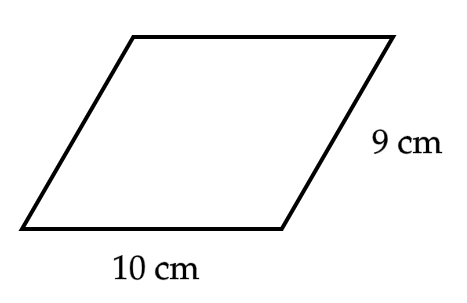
\includegraphics[scale=0.25]{pics/perimeter_1.png}
        \end{figure}
    \end{example}
    %
\end{frame}
%%%%%%%%%%%%%%%%%%%%%%%%%%%%%%%%%%%%%%%
%        SLIDE 
%%%%%%%%%%%%%%%%%%%%%%%%%%%%%%%%%%%%%%%
\section{Area}
\begin{frame}[t]{Area}
    \begin{columns}[t]
    %
    \column{0.45\textwidth}
    \begin{block}{Definition}
        An area, denoted $A$, is the measure of region within the boundaries of a shape.
    \end{block}
    %
    \begin{itemize}
        \item In other words, area is the size of surface insides a shape.
    \end{itemize}
    %
    \column{0.45\textwidth}
    \begin{figure}[H]
        \centering
        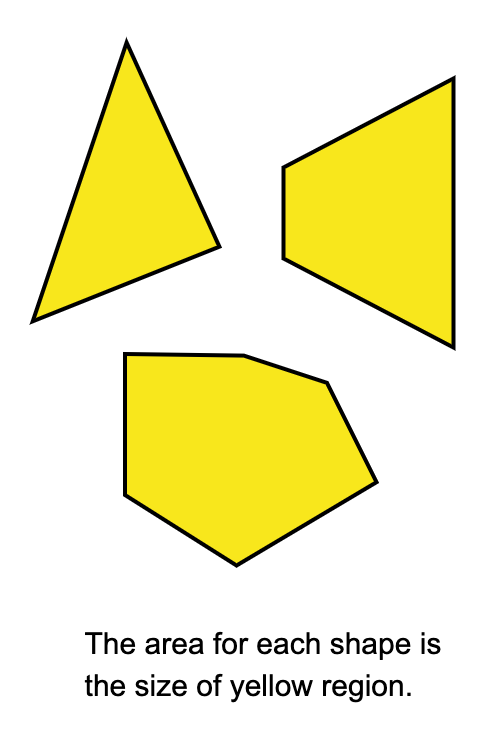
\includegraphics[width=0.6\textwidth]{pics/area_def.png}
    \end{figure}        
    \end{columns}
\end{frame}
%%%%%%%%%%%%%%%%%%%%%%%%%%%%%%%%%%%%%%%
%        SLIDE 
%%%%%%%%%%%%%%%%%%%%%%%%%%%%%%%%%%%%%%%
\subsection{How to Measure the Area?}
\begin{frame}{How to Measure the Area?}
    \begin{itemize}
        \item Area is basically the number of \textit{square units} that covers a shape.
    \end{itemize}
    %
    \begin{figure}[H]
        \centering
        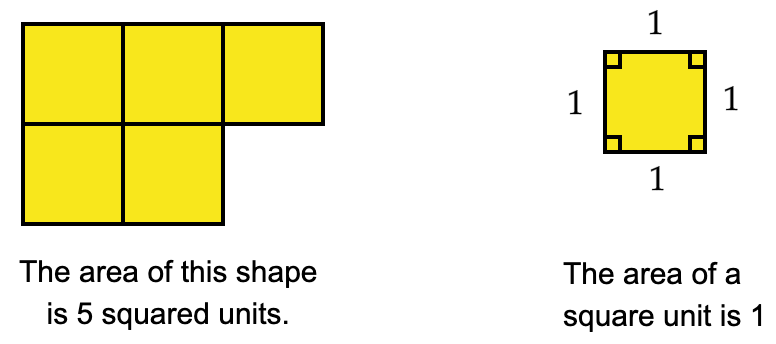
\includegraphics[scale=0.3]{pics/square_units.png}
    \end{figure}
    %
    \begin{itemize}
        \item The area is measure in squared units like square inches ($\mathrm{in^2}$), squared feet ($\mathrm{ft^2}$), squared cm ($\mathrm{cm^2}$), and so on.
        \item Using square units, we eventually develop a formula to calculate the area.
    \end{itemize}
\end{frame}
%%%%%%%%%%%%%%%%%%%%%%%%%%%%%%%%%%%%%%%
%        SLIDE 
%%%%%%%%%%%%%%%%%%%%%%%%%%%%%%%%%%%%%%%
\subsection{Area of a Rectangle}
\begin{frame}[t]{Area of a Rectangle}
    \begin{columns}[t]
    \column{0.45\textwidth}
    \begin{itemize}
        \item To find the area of a rectangle, we will find it using the square units. 
        \item As it is shown in Figure on the right, there is a relationship between the area of a rectangle, its length ($\ell$), and its width ($w$).
    \end{itemize}
    %
    \begin{block}{Formula}
        The area of a rectangle with length $\ell$ and width $w$ is equal to
        \[ A = \ell\cdot w \]
    \end{block}
    %
    \column{0.45\textwidth}
    %
    \begin{figure}[H]
        \centering
        

\tikzset{every picture/.style={line width=0.75pt}} %set default line width to 0.75pt        

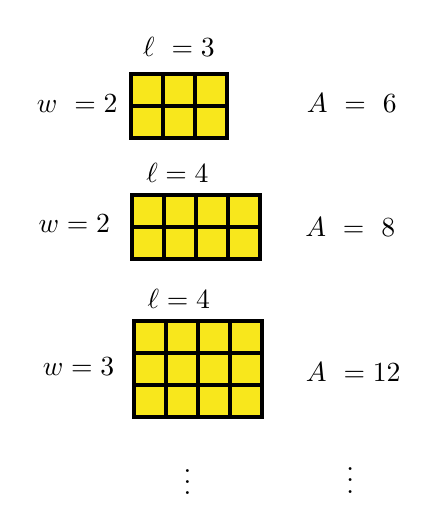
\begin{tikzpicture}[x=0.75pt,y=0.75pt,yscale=-1,xscale=1,scale=0.7]
%uncomment if require: \path (0,338); %set diagram left start at 0, and has height of 338

%Shape: Square [id:dp38271822688596946] 
\draw  [fill={rgb, 255:red, 248; green, 231; blue, 28 }  ,fill opacity=1 ][line width=1.5]  (189,34) -- (211,34) -- (211,56) -- (189,56) -- cycle ;
%Shape: Square [id:dp8679439248883813] 
\draw  [fill={rgb, 255:red, 248; green, 231; blue, 28 }  ,fill opacity=1 ][line width=1.5]  (211,34) -- (233,34) -- (233,56) -- (211,56) -- cycle ;
%Shape: Square [id:dp3558050933364425] 
\draw  [fill={rgb, 255:red, 248; green, 231; blue, 28 }  ,fill opacity=1 ][line width=1.5]  (233,34) -- (255,34) -- (255,56) -- (233,56) -- cycle ;
%Shape: Square [id:dp8748116538918442] 
\draw  [fill={rgb, 255:red, 248; green, 231; blue, 28 }  ,fill opacity=1 ][line width=1.5]  (189,56) -- (211,56) -- (211,78) -- (189,78) -- cycle ;
%Shape: Square [id:dp06759803167989387] 
\draw  [fill={rgb, 255:red, 248; green, 231; blue, 28 }  ,fill opacity=1 ][line width=1.5]  (211,56) -- (233,56) -- (233,78) -- (211,78) -- cycle ;
%Shape: Square [id:dp3172857824306643] 
\draw  [fill={rgb, 255:red, 248; green, 231; blue, 28 }  ,fill opacity=1 ][line width=1.5]  (233,56) -- (255,56) -- (255,78) -- (233,78) -- cycle ;
%Shape: Square [id:dp9771058827150725] 
\draw  [fill={rgb, 255:red, 248; green, 231; blue, 28 }  ,fill opacity=1 ][line width=1.5]  (190,117) -- (212,117) -- (212,139) -- (190,139) -- cycle ;
%Shape: Square [id:dp10490248151810566] 
\draw  [fill={rgb, 255:red, 248; green, 231; blue, 28 }  ,fill opacity=1 ][line width=1.5]  (212,117) -- (234,117) -- (234,139) -- (212,139) -- cycle ;
%Shape: Square [id:dp8310609107018645] 
\draw  [fill={rgb, 255:red, 248; green, 231; blue, 28 }  ,fill opacity=1 ][line width=1.5]  (234,117) -- (256,117) -- (256,139) -- (234,139) -- cycle ;
%Shape: Square [id:dp5473468611089647] 
\draw  [fill={rgb, 255:red, 248; green, 231; blue, 28 }  ,fill opacity=1 ][line width=1.5]  (190,139) -- (212,139) -- (212,161) -- (190,161) -- cycle ;
%Shape: Square [id:dp12474790550517523] 
\draw  [fill={rgb, 255:red, 248; green, 231; blue, 28 }  ,fill opacity=1 ][line width=1.5]  (212,139) -- (234,139) -- (234,161) -- (212,161) -- cycle ;
%Shape: Square [id:dp34696767252717375] 
\draw  [fill={rgb, 255:red, 248; green, 231; blue, 28 }  ,fill opacity=1 ][line width=1.5]  (234,139) -- (256,139) -- (256,161) -- (234,161) -- cycle ;
%Shape: Square [id:dp13867107777486232] 
\draw  [fill={rgb, 255:red, 248; green, 231; blue, 28 }  ,fill opacity=1 ][line width=1.5]  (256,117) -- (278,117) -- (278,139) -- (256,139) -- cycle ;
%Shape: Square [id:dp5849236655713153] 
\draw  [fill={rgb, 255:red, 248; green, 231; blue, 28 }  ,fill opacity=1 ][line width=1.5]  (256,139) -- (278,139) -- (278,161) -- (256,161) -- cycle ;
%Shape: Square [id:dp7422021146428393] 
\draw  [fill={rgb, 255:red, 248; green, 231; blue, 28 }  ,fill opacity=1 ][line width=1.5]  (191,204) -- (213,204) -- (213,226) -- (191,226) -- cycle ;
%Shape: Square [id:dp8646869287162122] 
\draw  [fill={rgb, 255:red, 248; green, 231; blue, 28 }  ,fill opacity=1 ][line width=1.5]  (213,204) -- (235,204) -- (235,226) -- (213,226) -- cycle ;
%Shape: Square [id:dp436268216442143] 
\draw  [fill={rgb, 255:red, 248; green, 231; blue, 28 }  ,fill opacity=1 ][line width=1.5]  (235,204) -- (257,204) -- (257,226) -- (235,226) -- cycle ;
%Shape: Square [id:dp40039453862710905] 
\draw  [fill={rgb, 255:red, 248; green, 231; blue, 28 }  ,fill opacity=1 ][line width=1.5]  (191,226) -- (213,226) -- (213,248) -- (191,248) -- cycle ;
%Shape: Square [id:dp34900812081397414] 
\draw  [fill={rgb, 255:red, 248; green, 231; blue, 28 }  ,fill opacity=1 ][line width=1.5]  (213,226) -- (235,226) -- (235,248) -- (213,248) -- cycle ;
%Shape: Square [id:dp6134216351528443] 
\draw  [fill={rgb, 255:red, 248; green, 231; blue, 28 }  ,fill opacity=1 ][line width=1.5]  (235,226) -- (257,226) -- (257,248) -- (235,248) -- cycle ;
%Shape: Square [id:dp2972790637499185] 
\draw  [fill={rgb, 255:red, 248; green, 231; blue, 28 }  ,fill opacity=1 ][line width=1.5]  (257,204) -- (279,204) -- (279,226) -- (257,226) -- cycle ;
%Shape: Square [id:dp6141269163406937] 
\draw  [fill={rgb, 255:red, 248; green, 231; blue, 28 }  ,fill opacity=1 ][line width=1.5]  (257,226) -- (279,226) -- (279,248) -- (257,248) -- cycle ;
%Shape: Square [id:dp04871647434354265] 
\draw  [fill={rgb, 255:red, 248; green, 231; blue, 28 }  ,fill opacity=1 ][line width=1.5]  (191,248) -- (213,248) -- (213,270) -- (191,270) -- cycle ;
%Shape: Square [id:dp6693543844606036] 
\draw  [fill={rgb, 255:red, 248; green, 231; blue, 28 }  ,fill opacity=1 ][line width=1.5]  (213,248) -- (235,248) -- (235,270) -- (213,270) -- cycle ;
%Shape: Square [id:dp25950883575769756] 
\draw  [fill={rgb, 255:red, 248; green, 231; blue, 28 }  ,fill opacity=1 ][line width=1.5]  (235,248) -- (257,248) -- (257,270) -- (235,270) -- cycle ;
%Shape: Square [id:dp5668503605566757] 
\draw  [fill={rgb, 255:red, 248; green, 231; blue, 28 }  ,fill opacity=1 ][line width=1.5]  (257,248) -- (279,248) -- (279,270) -- (257,270) -- cycle ;

% Text Node
\draw (222,15) node   {$\ell \ =3$};
% Text Node
\draw (152,54) node   {$w\ =2$};
% Text Node
\draw (341,54) node   {$A\ =\ 6$};
% Text Node
\draw (221,102) node   {$\ell =4$};
% Text Node
\draw (150,137) node   {$w=2$};
% Text Node
\draw (340,139) node   {$A\ =\ 8$};
% Text Node
\draw (222,189) node   {$\ell =4$};
% Text Node
\draw (153,235) node   {$w=3$};
% Text Node
\draw (342,239) node   {$A\ =12$};
% Text Node
\draw (228,309) node   {$\boldsymbol{\vdots }$};
% Text Node
\draw (340,308) node   {$\boldsymbol{\vdots }$};


\end{tikzpicture}
    \end{figure}
    \end{columns}
\end{frame}
%%%%%%%%%%%%%%%%%%%%%%%%%%%%%%%%%%%%%%%
%        SLIDE 
%%%%%%%%%%%%%%%%%%%%%%%%%%%%%%%%%%%%%%%
\subsection{Area of a Square}
\begin{frame}[t]{Area of a Square}
    \begin{columns}
    \column{0.45\textwidth}
    \begin{itemize}
        \item A square is a special case of a rectangle in which both length and width are equal in length.
        \item Let's say they both are equal to $s$.
        \item Using the rectangle formula, one can easily find the area of a square.
    \end{itemize}
    %
    \begin{block}{Formula}
        If a side of square is $s$, then its area can be found as follow:
        \[ A = s^2\]
    \end{block}
    %
    \column{0.45\textwidth}
    \begin{figure}[H]
        \centering
        

\tikzset{every picture/.style={line width=0.75pt}} %set default line width to 0.75pt        

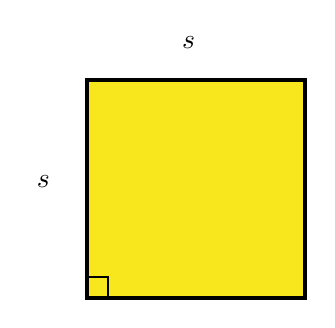
\begin{tikzpicture}[x=0.75pt,y=0.75pt,yscale=-1,xscale=1]
%uncomment if require: \path (0,167); %set diagram left start at 0, and has height of 167

%Shape: Square [id:dp9958510811050907] 
\draw  [fill={rgb, 255:red, 248; green, 231; blue, 28 }  ,fill opacity=1 ][line width=1.5]  (207,37) -- (312,37) -- (312,142) -- (207,142) -- cycle ;
%Shape: Square [id:dp2209502611968972] 
\draw   (207,132) -- (217,132) -- (217,142) -- (207,142) -- cycle ;

% Text Node
\draw (186,86) node   {$s$};
% Text Node
\draw (256,19) node   {$s$};
% Text Node
% \draw (411,87) node   {$ \begin{array}{l}
% \boldsymbol{A\ =\ s^{2}}\\
% \\
% \boldsymbol{P\ =\ 4s}
% \end{array}$};


\end{tikzpicture}
    \end{figure}    
    \end{columns}
\end{frame}
%%%%%%%%%%%%%%%%%%%%%%%%%%%%%%%%%%%%%%%
%        SLIDE 
%%%%%%%%%%%%%%%%%%%%%%%%%%%%%%%%%%%%%%%
\begin{frame}[t]{Example (Find Area and Perimeter)}
    \begin{example}
        Find the area and perimeter of each shape.
        %
        \begin{figure}[H]
            \centering
            

\tikzset{every picture/.style={line width=0.75pt}} %set default line width to 0.75pt        

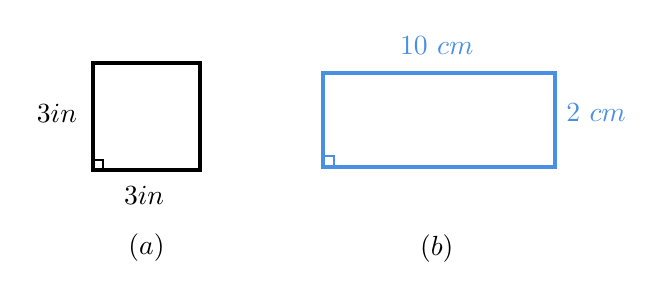
\begin{tikzpicture}[x=0.75pt,y=0.75pt,yscale=-1,xscale=1, scale=0.6]
%uncomment if require: \path (0,218); %set diagram left start at 0, and has height of 218

%Shape: Square [id:dp9958510811050907] 
\draw  [line width=1.5]  (135,45) -- (221,45) -- (221,131) -- (135,131) -- cycle ;
%Shape: Square [id:dp2209502611968972] 
\draw   (135,122.81) -- (143.19,122.81) -- (143.19,131) -- (135,131) -- cycle ;
%Shape: Rectangle [id:dp27912537729912623] 
\draw  [color={rgb, 255:red, 74; green, 144; blue, 226 }  ,draw opacity=1 ][line width=1.5]  (320,53) -- (506,53) -- (506,128) -- (320,128) -- cycle ;
%Shape: Square [id:dp059563169319218456] 
\draw  [color={rgb, 255:red, 74; green, 144; blue, 226 }  ,draw opacity=1 ] (320,119.81) -- (328.19,119.81) -- (328.19,128) -- (320,128) -- cycle ;

% Text Node
\draw (106,85) node   {$3\text{ in}$};
% Text Node
\draw (176,151) node   {$3\text{ in}$};
% Text Node
\draw (178,193) node   {$( a)$};
% Text Node
\draw (411,31) node   {$\textcolor[rgb]{0.29,0.56,0.89}{10\ \text{cm}}$};
% Text Node
\draw (539,85) node   {$\textcolor[rgb]{0.29,0.56,0.89}{2\ }\textcolor[rgb]{0.29,0.56,0.89}{\text{cm}}$};
% Text Node
\draw (411,194) node   {$( b)$};


\end{tikzpicture}
        \end{figure}
    \end{example}
\end{frame}

%%%%%%%%%%%%%%%%%%%%%%%%%%%%%%%%%%%%%%%
%        SLIDE 
%%%%%%%%%%%%%%%%%%%%%%%%%%%%%%%%%%%%%%%
\subsection{Area of a Parallelogram}
\begin{frame}{Area of a Parallelogram}
    \begin{columns}
    %
    \column{0.45\textwidth}
    \begin{itemize}
        \item Height of a parallelogram, $h$, is the distance between two parallel sides.
        \item Those parallel sides are called bases and we showed them with $b$.
        \item It can be proven the area of a parallelogram is height times its base.
    \end{itemize}
    %
    \begin{block}{Formula}
        If $h$ is height of the parallelogram and $b$ is the side which height is perpendicular to it, then the area of the parallelogram can be found as follow:
        \[ A = b \cdot h\] 
    \end{block}
    %
    \column{0.45\textwidth}
    \begin{figure}[H]
        \centering
        

\tikzset{every picture/.style={line width=0.75pt}} %set default line width to 0.75pt        

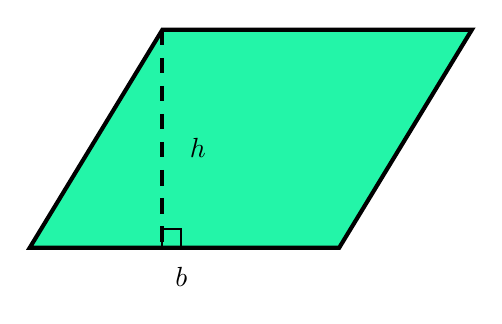
\begin{tikzpicture}[x=0.75pt,y=0.75pt,yscale=-1,xscale=1]
%uncomment if require: \path (0,187); %set diagram left start at 0, and has height of 187

%Shape: Parallelogram [id:dp6701686139689902] 
\draw  [fill={rgb, 255:red, 35; green, 245; blue, 168 }   ,fill opacity=1 ][line width=1.5]  (276.9,48) -- (426,48) -- (362.1,153) -- (213,153) -- cycle ;
%Straight Lines [id:da38364165600367084] 
\draw [line width=1.5]  [dash pattern={on 5.63pt off 4.5pt}]  (276.9,48) -- (276.9,153) ;


%Shape: Square [id:dp885829648238055] 
\draw   (276.9,144) -- (285.9,144) -- (285.9,153) -- (276.9,153) -- cycle ;

% Text Node
\draw (286,167) node   {$b$};
% Text Node
\draw (294,105) node   {$h$};


\end{tikzpicture}
    \end{figure}
    \end{columns}
\end{frame}
%%%%%%%%%%%%%%%%%%%%%%%%%%%%%%%%%%%%%%%
%        SLIDE 
%%%%%%%%%%%%%%%%%%%%%%%%%%%%%%%%%%%%%%%
\subsection{Area of a Triangle}
\begin{frame}{Area of a Triangle}
    \begin{columns}
    \column{0.45\textwidth}
        \begin{itemize}
            \item Two triangle make a parallelogram. 
            \item So the area of a triangle is half of a parallelogram with same base and height.
        \end{itemize}
        %
        \begin{block}{Formula}
            If $h$ is distance from one vertex to the side $b$ (called base), then the area of a triangle can be found using the following formula:
            \[  A = \frac{b\cdot h}{2} \]
        \end{block}
        %
        \column{0.45\textwidth}
    \begin{figure}[H]
        \centering
        

\tikzset{every picture/.style={line width=0.75pt}} %set default line width to 0.75pt        

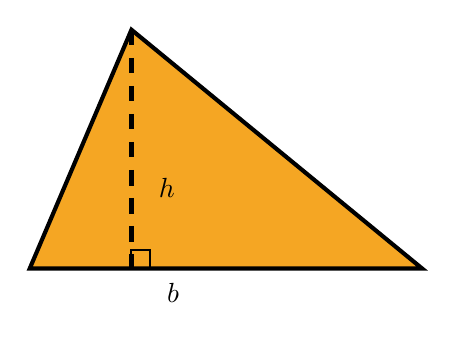
\begin{tikzpicture}[x=0.75pt,y=0.75pt,yscale=-1,xscale=1]
%uncomment if require: \path (0,200); %set diagram left start at 0, and has height of 200

%Shape: Triangle [id:dp48354767803270016] 
\draw  [fill={rgb, 255:red, 245; green, 166; blue, 35 }  ,fill opacity=1 ][line width=1.5]  (277,45) -- (417,160) -- (228,160) -- cycle ;
%Straight Lines [id:da38364165600367084] 
\draw [line width=1.5]  [dash pattern={on 5.63pt off 4.5pt}]  (277,45) -- (277,160) ;


%Shape: Square [id:dp885829648238055] 
\draw   (277,151) -- (286,151) -- (286,160) -- (277,160) -- cycle ;

% Text Node
\draw (297,172) node   {$b$};
% Text Node
\draw (294,121) node   {$h$};
% Text Node


\end{tikzpicture}
    \end{figure}        
    \end{columns}
\end{frame}
%%%%%%%%%%%%%%%%%%%%%%%%%%%%%%%%%%%%%%%
%        SLIDE 
%%%%%%%%%%%%%%%%%%%%%%%%%%%%%%%%%%%%%%%
\begin{frame}{Area of a Triangle (Cont'd)}
    \begin{itemize}
        \item For right triangle, we can consider on leg as a height and the other leg as a base (Figure a).
        \item In addition, one can draw a perpendicular line to the hypotenuse. In this case, the perpendicular line is our height and hypotenuse is our base (Figure b)
    \end{itemize}
    %
    \begin{figure}[H]
        \centering
        

\tikzset{every picture/.style={line width=0.75pt}} %set default line width to 0.75pt        

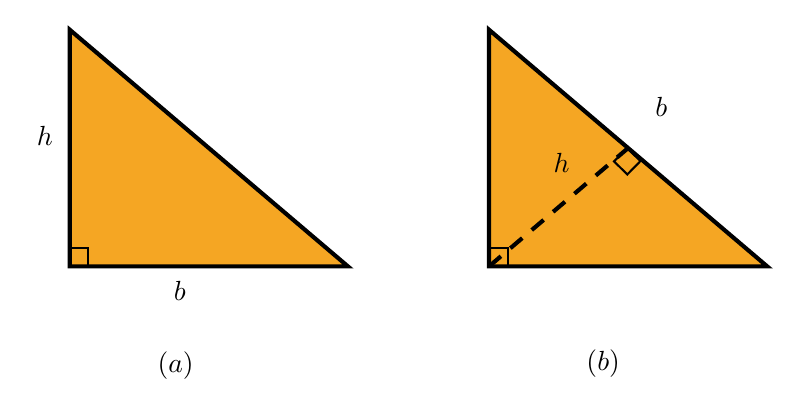
\begin{tikzpicture}[x=0.75pt,y=0.75pt,yscale=-1,xscale=1]
%uncomment if require: \path (0,256); %set diagram left start at 0, and has height of 256

%Shape: Right Triangle [id:dp7083168248857548] 
\draw  [fill={rgb, 255:red, 245; green, 166; blue, 35 }  ,fill opacity=1 ][line width=1.5]  (178,68) -- (312,182) -- (178,182) -- cycle ;
%Shape: Square [id:dp9879546899101135] 
\draw   (178,173) -- (187,173) -- (187,182) -- (178,182) -- cycle ;
%Shape: Right Triangle [id:dp9630416737865424] 
\draw  [fill={rgb, 255:red, 245; green, 166; blue, 35 }  ,fill opacity=1 ][line width=1.5]  (380,68) -- (514,182) -- (380,182) -- cycle ;
%Shape: Square [id:dp12336196242449993] 
\draw   (380,173) -- (389,173) -- (389,182) -- (380,182) -- cycle ;
%Straight Lines [id:da207575097514602] 
\draw [line width=1.5]  [dash pattern={on 5.63pt off 4.5pt}]  (380,182) -- (447,125) ;


%Shape: Square [id:dp9229345478868127] 
\draw   (440.2,131.42) -- (446.5,124.99) -- (452.93,131.28) -- (446.63,137.71) -- cycle ;

% Text Node
\draw (231,194) node   {$b$};
% Text Node
\draw (166,119) node   {$h$};;
% Text Node
\draw (463,105) node   {$b$};
% Text Node
\draw (415,132) node   {$h$};
% Text Node
\draw (229,230) node   {$( a)$};
% Text Node
\draw (435,229) node   {$( b)$};


\end{tikzpicture}
    \end{figure} 
\end{frame}
%%%%%%%%%%%%%%%%%%%%%%%%%%%%%%%%%%%%%%%
%        SLIDE 
%%%%%%%%%%%%%%%%%%%%%%%%%%%%%%%%%%%%%%%
\begin{frame}[t]{Example (Find Area)}
    \begin{example}
        Find the area of each shape.
        %
        \begin{figure}[H]
            \centering
            

\tikzset{every picture/.style={line width=0.75pt}} %set default line width to 0.75pt        

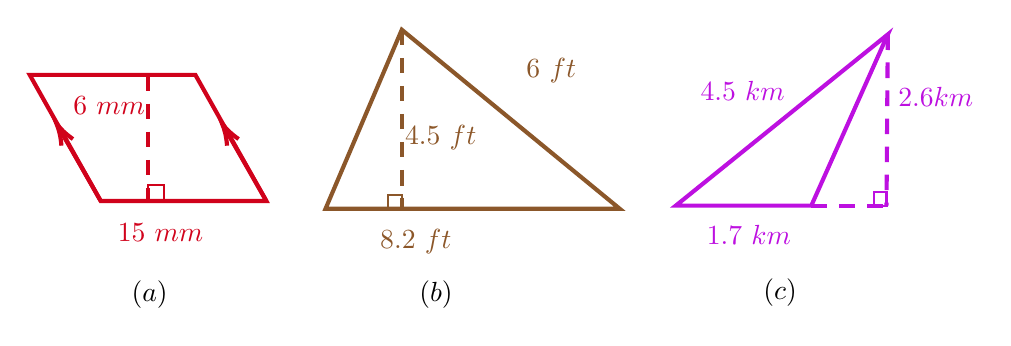
\begin{tikzpicture}[x=0.75pt,y=0.75pt,yscale=-1,xscale=1, scale=0.75]
%uncomment if require: \path (0,230); %set diagram left start at 0, and has height of 230

%Shape: Parallelogram [id:dp4045973963325873] 
\draw  [color={rgb, 255:red, 208; green, 2; blue, 27 }  ,draw opacity=1 ][line width=1.5]  (147.4,59) -- (41,59) -- (86.6,140) -- (193,140) -- cycle ;
%Straight Lines [id:da9796665582380797] 
\draw [color={rgb, 255:red, 208; green, 2; blue, 27 }  ,draw opacity=1 ][line width=1.5]  [dash pattern={on 5.63pt off 4.5pt}]  (117,59.5) -- (117,139.5) ;


%Shape: Square [id:dp06920862972284914] 
\draw  [color={rgb, 255:red, 208; green, 2; blue, 27 }  ,draw opacity=1 ] (117,129.5) -- (127,129.5) -- (127,139.5) -- (117,139.5) -- cycle ;
%Shape: Triangle [id:dp08961522547508038] 
\draw  [color={rgb, 255:red, 139; green, 87; blue, 42 }  ,draw opacity=1 ][line width=1.5]  (280,30) -- (420,145) -- (231,145) -- cycle ;
%Straight Lines [id:da8427678719260143] 
\draw [color={rgb, 255:red, 139; green, 87; blue, 42 }  ,draw opacity=1 ][line width=1.5]  [dash pattern={on 5.63pt off 4.5pt}]  (280,30) -- (280,145) ;


%Shape: Square [id:dp08529804115971995] 
\draw  [color={rgb, 255:red, 139; green, 87; blue, 42 }  ,draw opacity=1 ] (271,136) -- (280,136) -- (280,145) -- (271,145) -- cycle ;
%Shape: Polygon [id:ds9967185060442834] 
\draw  [color={rgb, 255:red, 189; green, 16; blue, 224 }  ,draw opacity=1 ][line width=1.5]  (456,143) -- (543.08,143) -- (592.22,33) -- cycle ;
%Straight Lines [id:da1558061082869422] 
\draw [color={rgb, 255:red, 189; green, 16; blue, 224 }  ,draw opacity=1 ][line width=1.5]  [dash pattern={on 5.63pt off 4.5pt}]  (592.22,33) -- (591.36,143) ;


%Straight Lines [id:da7378491629676467] 
\draw [color={rgb, 255:red, 189; green, 16; blue, 224 }  ,draw opacity=1 ][line width=1.5]  [dash pattern={on 5.63pt off 4.5pt}]  (543.08,143) -- (591.36,143) ;


%Shape: Rectangle [id:dp5477304566759069] 
\draw  [color={rgb, 255:red, 189; green, 16; blue, 224 }  ,draw opacity=1 ] (591.36,134) -- (583.6,134) -- (583.6,143) -- (591.36,143) -- cycle ;
%Straight Lines [id:da6859428859669638] 
\draw [color={rgb, 255:red, 208; green, 2; blue, 27 }  ,draw opacity=1 ][line width=1.5]    (86.6,140) -- (59.49,92.6) ;
\draw [shift={(58,90)}, rotate = 420.23] [color={rgb, 255:red, 208; green, 2; blue, 27 }  ,draw opacity=1 ][line width=1.5]    (14.21,-4.28) .. controls (9.04,-1.82) and (4.3,-0.39) .. (0,0) .. controls (4.3,0.39) and (9.04,1.82) .. (14.21,4.28)   ;

%Straight Lines [id:da26032096428140505] 
\draw [color={rgb, 255:red, 208; green, 2; blue, 27 }  ,draw opacity=1 ][line width=1.5]    (193,140) -- (165.89,92.6) ;
\draw [shift={(164.4,90)}, rotate = 420.23] [color={rgb, 255:red, 208; green, 2; blue, 27 }  ,draw opacity=1 ][line width=1.5]    (14.21,-4.28) .. controls (9.04,-1.82) and (4.3,-0.39) .. (0,0) .. controls (4.3,0.39) and (9.04,1.82) .. (14.21,4.28)   ;


% Text Node
\draw (92,79) node   {$\textcolor[rgb]{0.82,0.01,0.11}{6\ \text{mm}}$};
% Text Node
\draw (125,160) node   {$\textcolor[rgb]{0.82,0.01,0.11}{15\ }\textcolor[rgb]{0.82,0.01,0.11}{\text{mm}}$};
% Text Node
\draw (118,200) node   {$( a)$};
% Text Node
\draw (289,166) node   {$\textcolor[rgb]{0.55,0.34,0.16}{8.2\ \text{ ft}}$};
% Text Node
\draw (305,99) node   {$\textcolor[rgb]{0.55,0.34,0.16}{4.5\ \text{ft}}$};
% Text Node
\draw (376,56) node [color={rgb, 255:red, 139; green, 87; blue, 42 }  ,opacity=1 ]  {$6\ \text{ft}$};
% Text Node
\draw (302,200) node   {$( b)$};
% Text Node
\draw (503,162) node [color={rgb, 255:red, 189; green, 16; blue, 224 }  ,opacity=1 ]  {$1.7\ \text{km}$};
% Text Node
\draw (623,73) node [color={rgb, 255:red, 189; green, 16; blue, 224 }  ,opacity=1 ]  {$2.6\text{ km}$};
% Text Node
\draw (499,69) node [color={rgb, 255:red, 189; green, 16; blue, 224 }  ,opacity=1 ]  {$4.5\ \text{km}$};
% Text Node
\draw (523,199) node   {$( c)$};


\end{tikzpicture}
        \end{figure}
    \end{example}
\end{frame}
%%%%%%%%%%%%%%%%%%%%%%%%%%%%%%%%%%%%%%%
%        SLIDE 
%%%%%%%%%%%%%%%%%%%%%%%%%%%%%%%%%%%%%%%
\subsection{Area of a Trapezoid}
\begin{frame}{Area of a Trapezoid}
    \begin{columns}
    \column{0.45\textwidth}
        \begin{itemize}
            \item In trapezoid, the two parallel sides are called bases. It is usually denoted as $b_1$ and $b_2$.
            \item The distance between two bases is the height of the trapezoid, $h$.
        \end{itemize}
        %
        \begin{block}{Formula}
            The area of a trapezoid with bases $b_1$ and $b_2$ and height of $h$ can be found as follow:
            \[ A = \frac{(b_1+b_2)\cdot h}{2}\]
        \end{block}
    \column{0.45\textwidth}
        \begin{figure}[H]
            \centering
            

\tikzset{every picture/.style={line width=0.75pt}} %set default line width to 0.75pt        

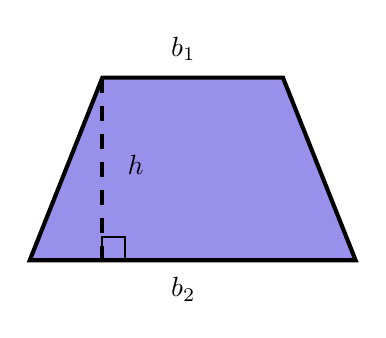
\begin{tikzpicture}[x=0.75pt,y=0.75pt,yscale=-1,xscale=1]
%uncomment if require: \path (0,153); %set diagram left start at 0, and has height of 153

%Shape: Trapezoid [id:dp6397225193899372] 
\draw  [fill={rgb, 255:red, 153; green, 144; blue, 235 }  ,fill opacity=1 ][line width=1.5]  (187,121) -- (222,33) -- (309,33) -- (344,121) -- cycle ;
%Straight Lines [id:da3353080959428809] 
\draw [line width=1.5]  [dash pattern={on 5.63pt off 4.5pt}]  (222,33) -- (222,121) ;


%Shape: Square [id:dp5126106092503966] 
\draw   (222,110) -- (233,110) -- (233,121) -- (222,121) -- cycle ;

% Text Node
\draw (261,19) node   {$b_{1}$};
% Text Node
\draw (261,135) node   {$b_{2}$};
% Text Node
\draw (238,75) node   {$h$};


\end{tikzpicture}
        \end{figure}
    \end{columns}
\end{frame}
%%%%%%%%%%%%%%%%%%%%%%%%%%%%%%%%%%%%%%%
%        SLIDE 
%%%%%%%%%%%%%%%%%%%%%%%%%%%%%%%%%%%%%%%
\begin{frame}[t]{Example (Find the Area)}
    \begin{example}
        Find the area of a below trapezoid.
        %
        \begin{figure}[H]
            \centering
            

\tikzset{every picture/.style={line width=0.75pt}} %set default line width to 0.75pt        

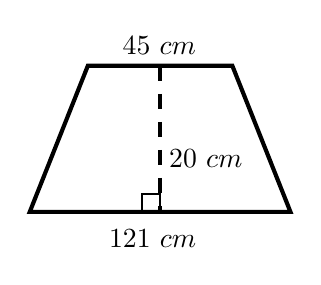
\begin{tikzpicture}[x=0.75pt,y=0.75pt,yscale=-1,xscale=1, scale=0.8]
%uncomment if require: \path (0,145); %set diagram left start at 0, and has height of 145

%Shape: Trapezoid [id:dp28634609077041273] 
\draw  [line width=1.5]  (243,109) -- (278,21) -- (365,21) -- (400,109) -- cycle ;
%Straight Lines [id:da16123629658218785] 
\draw [line width=1.5]  [dash pattern={on 5.63pt off 4.5pt}]  (321.5,21) -- (321.5,109) ;


%Shape: Square [id:dp7708997304192546] 
\draw   (310.5,98) -- (321.5,98) -- (321.5,109) -- (310.5,109) -- cycle ;

% Text Node
\draw (317,125) node   {$121\ \text{cm}$};
% Text Node
\draw (349,77) node   {$20\ \text{cm}$};
% Text Node
\draw (321,9) node   {$45\ \text{cm}$};


\end{tikzpicture}
        \end{figure}
    \end{example}
\end{frame}
%%%%%%%%%%%%%%%%%%%%%%%%%%%%%%%%%%%%%%%
%        SLIDE 
%%%%%%%%%%%%%%%%%%%%%%%%%%%%%%%%%%%%%%%
\section{More on Right Triangles}
\subsection{Pythagorean Theorem}
\begin{frame}[t]{Pythagorean Theorem}
    \begin{columns}[t]
    \column{0.45\textwidth}
        \begin{itemize}
            \item The Theorem of Pythagoras or Pythagorean theorem is a well-known theorem. 
            \item The theorem makes reference to a right triangle.
            \item As you might remember, The side opposite the right angle is the longest side and is called the hypotenuse.
        \end{itemize}
        %
    \column{0.45\textwidth}
        %
        \begin{block}{Formula}
            In a right triangle, the sum of the squares of the two right-angle sides (legs) will always be the same as the square of the hypotenuse. In symbol form:
            \[a^2+b^2 = c^2\]
        \end{block}
        %
        \begin{figure}[H]
            \centering
            \tikzset{every picture/.style={line width=0.75pt}} %set default line width to 0.75pt        
            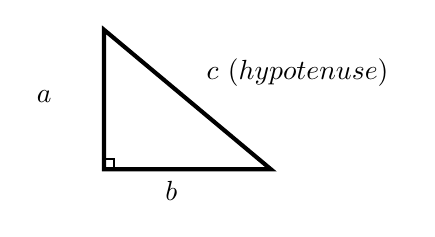
\begin{tikzpicture}[x=0.75pt,y=0.75pt,yscale=-1,xscale=1,scale=0.6]
            \draw  [line width=1.5]  (276,25) -- (410,137) -- (276,137) -- cycle ;
            \draw   (276,129) -- (284,129) -- (284,137) -- (276,137) -- cycle ;
            % Text Node
            \draw (228,79) node   {$a$};
            % Text Node
            \draw (330,154) node  {$b$};
            % Text Node
            \draw (350,59) node[right=0.1pt]   {$c\ \text{(hypotenuse)} \ $};
            \end{tikzpicture}
        \end{figure}
    \end{columns}
\end{frame}
%%%%%%%%%%%%%%%%%%%%%%%%%%%%%%%%%%%%%%%
%        SLIDE 
%%%%%%%%%%%%%%%%%%%%%%%%%%%%%%%%%%%%%%%
\begin{frame}[t]{Example (Find the missing side)}
    \begin{example}
        Find the missing side in each triangle.
        %
        \begin{figure}[H]
            \centering
            

\tikzset{every picture/.style={line width=0.75pt}} %set default line width to 0.75pt        

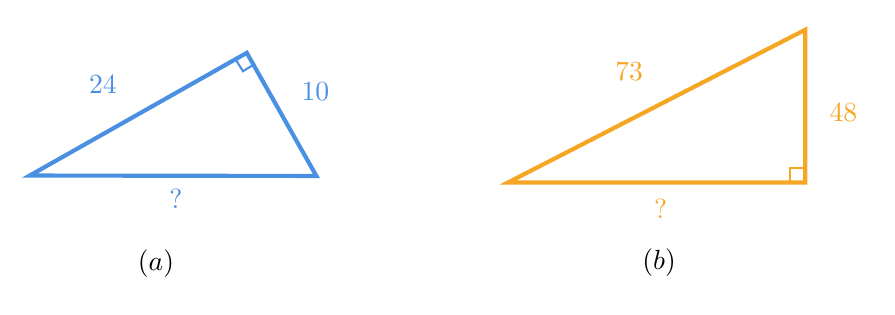
\begin{tikzpicture}[x=0.75pt,y=0.75pt,yscale=-1,xscale=1, scale=0.8]
%uncomment if require: \path (0,207); %set diagram left start at 0, and has height of 207

%Shape: Right Triangle [id:dp12946886895490128] 
\draw  [color={rgb, 255:red, 74; green, 144; blue, 226 }  ,draw opacity=1 ][line width=1.5]  (238.59,126.05) -- (65.98,125.8) -- (196.68,51.92) -- cycle ;
%Shape: Square [id:dp2641846486111634] 
\draw  [color={rgb, 255:red, 74; green, 144; blue, 226 }  ,draw opacity=1 ] (197,51.98) -- (201.19,58.8) -- (194.37,62.98) -- (190.18,56.17) -- cycle ;
%Shape: Right Triangle [id:dp9891393970753262] 
\draw  [color={rgb, 255:red, 245; green, 166; blue, 35 }  ,draw opacity=1 ][line width=1.5]  (533,38) -- (354,130) -- (533,130) -- cycle ;
%Shape: Square [id:dp34385770558966033] 
\draw  [color={rgb, 255:red, 245; green, 166; blue, 35 }  ,draw opacity=1 ] (524,121) -- (533,121) -- (533,130) -- (524,130) -- cycle ;

% Text Node
\draw (110,71) node   {$\textcolor[rgb]{0.29,0.56,0.89}{24}$};
% Text Node
\draw (238,75) node   {$\textcolor[rgb]{0.29,0.56,0.89}{10}$};
% Text Node
\draw (154,140) node   {$\textcolor[rgb]{0.29,0.56,0.89}{?}$};
% Text Node
\draw (427,63) node   {$\textcolor[rgb]{0.96,0.65,0.14}{73}$};
% Text Node
\draw (556,88) node   {$\textcolor[rgb]{0.96,0.65,0.14}{48}$};
% Text Node
\draw (446,146) node   {$\textcolor[rgb]{0.96,0.65,0.14}{?}$};
% Text Node
\draw (142,179) node   {$( a)$};
% Text Node
\draw (445,178) node   {$( b)$};


\end{tikzpicture}
        \end{figure}
    \end{example}   
\end{frame}
%%%%%%%%%%%%%%%%%%%%%%%%%%%%%%%%%%%%%%%
%        SLIDE 
%%%%%%%%%%%%%%%%%%%%%%%%%%%%%%%%%%%%%%%
\section{Circles}
\begin{frame}{Circles}
    \begin{itemize}
        \item A circle is a set of points that are the same distance from a fixed point.
        \item The fixed point is called center and we show it with letter $O$.
        \item A line segment from the center to a point on the circle is called radius denotes with $r$.
    \end{itemize}
    %
    \begin{figure}[H]
        \centering
        

\tikzset{every picture/.style={line width=0.75pt}} %set default line width to 0.75pt        

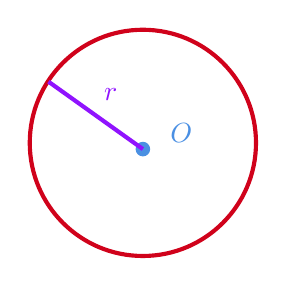
\begin{tikzpicture}[x=0.75pt,y=0.75pt,yscale=-1,xscale=1]
%uncomment if require: \path (0,140); %set diagram left start at 0, and has height of 140

%Shape: Circle [id:dp8118732481164563] 
\draw  [color={rgb, 255:red, 208; green, 2; blue, 27 }  ,draw opacity=1 ][line width=1.5]  (277,71.5) .. controls (277,41.4) and (301.4,17) .. (331.5,17) .. controls (361.6,17) and (386,41.4) .. (386,71.5) .. controls (386,101.6) and (361.6,126) .. (331.5,126) .. controls (301.4,126) and (277,101.6) .. (277,71.5) -- cycle ;
%Shape: Circle [id:dp14232976554180699] 
\draw  [color={rgb, 255:red, 74; green, 144; blue, 226 }  ,draw opacity=1 ][fill={rgb, 255:red, 74; green, 144; blue, 226 }  ,fill opacity=1 ] (328.5,74.5) .. controls (328.5,72.84) and (329.84,71.5) .. (331.5,71.5) .. controls (333.16,71.5) and (334.5,72.84) .. (334.5,74.5) .. controls (334.5,76.16) and (333.16,77.5) .. (331.5,77.5) .. controls (329.84,77.5) and (328.5,76.16) .. (328.5,74.5) -- cycle ;
%Straight Lines [id:da2079968527177969] 
\draw [color={rgb, 255:red, 144; green, 19; blue, 254 }  ,draw opacity=1 ][line width=1.5]    (286,42) -- (331.5,74.5) ;



% Text Node
\draw (350,67) node   {$\textcolor[rgb]{0.29,0.56,0.89}{O}$};
% Text Node
\draw (316,48) node   {$\textcolor[rgb]{0.56,0.07,1}{r}$};


\end{tikzpicture}
    \end{figure}
\end{frame}
%%%%%%%%%%%%%%%%%%%%%%%%%%%%%%%%%%%%%%%
%        SLIDE 
%%%%%%%%%%%%%%%%%%%%%%%%%%%%%%%%%%%%%%%
\begin{frame}{Circles (Cont'd)}
    \begin{itemize}
        \item The diameter, $d$, is a line segment passing though the center with endpoints on the circle.
        \[          r = \frac{d}{2}   \]
        \item Any other line segments with endpoints on the circle without passing though the center are called chords.
    \end{itemize}
    %
    \begin{figure}[H]
        \centering
        

\tikzset{every picture/.style={line width=0.75pt}} %set default line width to 0.75pt        

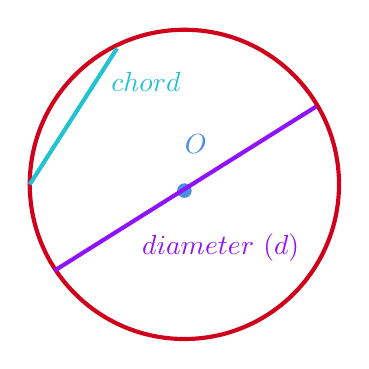
\begin{tikzpicture}[x=0.75pt,y=0.75pt,yscale=-1,xscale=1]
%uncomment if require: \path (0,188); %set diagram left start at 0, and has height of 188

%Shape: Circle [id:dp8118732481164563] 
\draw  [color={rgb, 255:red, 208; green, 2; blue, 27 }  ,draw opacity=1 ][line width=1.5]  (254,91.5) .. controls (254,50.35) and (287.35,17) .. (328.5,17) .. controls (369.65,17) and (403,50.35) .. (403,91.5) .. controls (403,132.65) and (369.65,166) .. (328.5,166) .. controls (287.35,166) and (254,132.65) .. (254,91.5) -- cycle ;
%Shape: Circle [id:dp14232976554180699] 
\draw  [color={rgb, 255:red, 74; green, 144; blue, 226 }  ,draw opacity=1 ][fill={rgb, 255:red, 74; green, 144; blue, 226 }  ,fill opacity=1 ] (325.83,93.13) .. controls (326.58,91.66) and (328.39,91.07) .. (329.87,91.83) .. controls (331.34,92.58) and (331.93,94.39) .. (331.17,95.87) .. controls (330.42,97.34) and (328.61,97.93) .. (327.13,97.17) .. controls (325.66,96.42) and (325.07,94.61) .. (325.83,93.13) -- cycle ;
%Straight Lines [id:da2079968527177969] 
\draw [color={rgb, 255:red, 144; green, 19; blue, 254 }  ,draw opacity=1 ][line width=1.5]    (266,133) -- (392,54) ;


%Straight Lines [id:da9513159212046638] 
\draw [color={rgb, 255:red, 33; green, 195; blue, 211 }  ,draw opacity=1 ][line width=1.5]    (296,26) -- (254,91.5) ;



% Text Node
\draw (334,72) node   {$\textcolor[rgb]{0.29,0.56,0.89}{O}$};
% Text Node
\draw (346,122) node   {$\textcolor[rgb]{0.56,0.07,1}{diameter\ ( d)}$};
% Text Node
\draw (310,42) node [color={rgb, 255:red, 33; green, 195; blue, 211 }  ,opacity=1 ]  {$\textcolor[rgb]{0.13,0.76,0.83}{chord}$};


\end{tikzpicture}
    \end{figure}
\end{frame}
%%%%%%%%%%%%%%%%%%%%%%%%%%%%%%%%%%%%%%%
%        SLIDE 
%%%%%%%%%%%%%%%%%%%%%%%%%%%%%%%%%%%%%%%
\subsection{Number \texorpdfstring{$\pi$}{TEXT} }
\begin{frame}{Number $\pi$}
    %
    \begin{itemize}
        \item \textit{Archimedes} was a Greek mathematician, physicist, engineer, and astronomer.
        \item He discovered that in any circle the ratio of circumference to diameter is always the same number $3.14159\cdots$
        \item It has been represented by the Greek letter $\pi$ since the mid-18th century, though it is also sometimes spelled out as ``pi''.
    \end{itemize}
    %
    \begin{figure}[H]
        \centering
        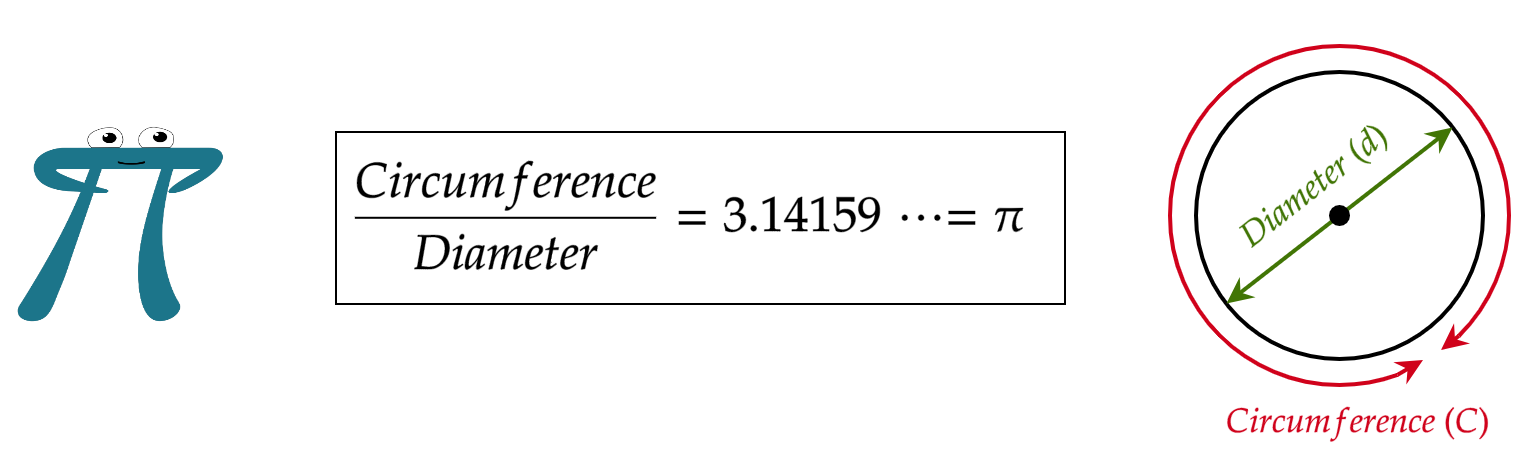
\includegraphics[scale=0.27]{pics/circumference_to_diameter.png}
    \end{figure}
\end{frame}
%%%%%%%%%%%%%%%%%%%%%%%%%%%%%%%%%%%%%%%
%        SLIDE 
%%%%%%%%%%%%%%%%%%%%%%%%%%%%%%%%%%%%%%%
\begin{frame}{Number $\pi$ (Cont'd)}
    \begin{columns}
    \column{0.45\textwidth}
    \begin{itemize}
        \item $\pi$ is a constant number.
        \item It is a irrational number since we cannot express it as a fraction.
        \item But its digits goes forever.
        \item In most cases, we leave our answers in terms of $\pi$ unless the problem itself give us some approximation.
    \end{itemize}
    %
    \column{0.45\textwidth}
    \begin{figure}[H]
        \centering
        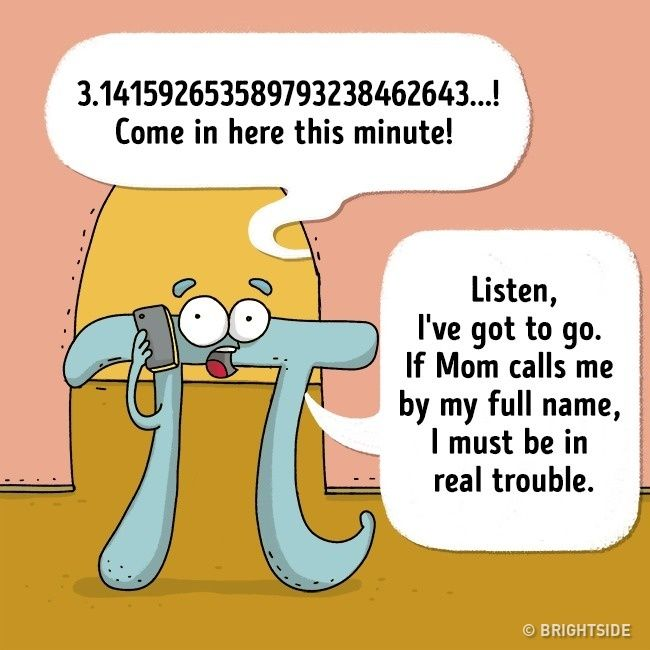
\includegraphics[scale=0.3]{pics/pi_funny.jpg}
    \end{figure}
    \end{columns}
\end{frame}
%%%%%%%%%%%%%%%%%%%%%%%%%%%%%%%%%%%%%%%
%        SLIDE 
%%%%%%%%%%%%%%%%%%%%%%%%%%%%%%%%%%%%%%%
\subsection{Circumference of a Circle}
\begin{frame}[t]{Circumference of a Circle}
    \begin{itemize}
        \item Circumference is denoted as $C$.
        \item We learned circumference divided by diameter is always equal to $\pi$.
        \item If we multiply both sides of the equation by $2r$, we will get an equation for $C$.
    \end{itemize}
    %
    \begin{columns}[t]
    \column{0.45\textwidth}
    \begin{block}{Circumference of a Circle}
        The circumference of a circle, $C$, with radius $r$ is
        \[ C = 2\pi r\]
    \end{block}
    %
    \column{0.45\textwidth}
    \begin{figure}[H]
        \centering
        
\includegraphics[scale=0.13]{pics/wow.jpg}
    \end{figure}
    \end{columns}
\end{frame}
%%%%%%%%%%%%%%%%%%%%%%%%%%%%%%%%%%%%%%%
%        SLIDE 
%%%%%%%%%%%%%%%%%%%%%%%%%%%%%%%%%%%%%%%
\subsection{Area of a Circle}
\begin{frame}[t]{Area of a Circle}
    %
    \begin{columns}
    \column{0.45\textwidth}
    \begin{itemize}
            \item \textit{Archimedes} also found the area of the circle by dividing circles into some sectors. 
            \item He then argued the area of those slices is the same as a right triangle whose is $2\pi r$ and its height $r$.
        \end{itemize}
    %
    \column{0.45\textwidth}
    \begin{block}{Area of a Circle}
        The area of a circle with radius $r$ is
        \[ A = \pi r^2\]
    \end{block}
    %
    \end{columns}
    %
    \begin{figure}
        \centering
        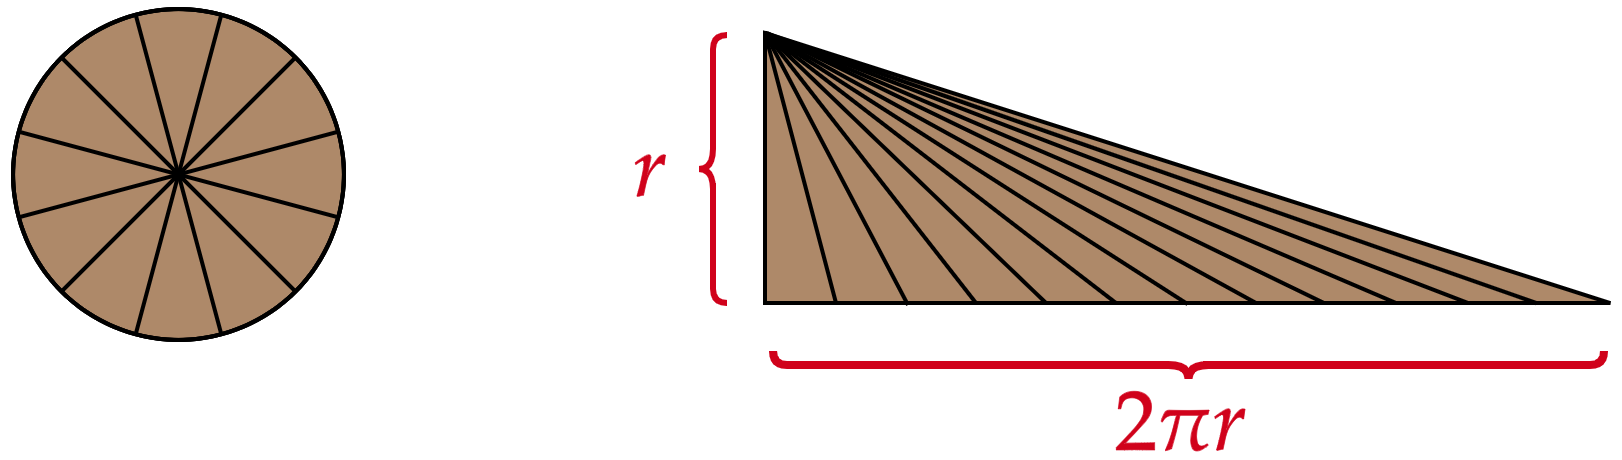
\includegraphics[scale=0.23]{pics/archimede_area.png}
    \end{figure}
\end{frame}
%%%%%%%%%%%%%%%%%%%%%%%%%%%%%%%%%%%%%%%
%        SLIDE 
%%%%%%%%%%%%%%%%%%%%%%%%%%%%%%%%%%%%%%%
\begin{frame}[t]{Example (Find Circumference and Area)}
    \begin{example}
        Find the circumference and area of a circle with diameter 12 cm.
    \end{example}
\end{frame}